\documentclass[a4paper,11pt,spanish,sans]{exam}
\usepackage[spanish]{babel}
%\usepackage[utf8]{inputenc}
\usepackage{multicol}
%\usepackage[latin1]{inputenc}
\usepackage{fontspec}%la posta para las tildes con lualatex
\usepackage[margin=0.5in]{geometry}
\usepackage{amsmath,amssymb}
\usepackage{multicol}
\usepackage{natbib}
\usepackage{graphicx}
\usepackage{hyperref}
\usepackage{epstopdf}
\usepackage{capt-of}
\usepackage{gensymb}
\usepackage{wrapfig}
%\usepackage{animate}
\usepackage[usenames]{color}
\usepackage{tikz}%para graficos
\usetikzlibrary{decorations.markings}
\usetikzlibrary{shapes.geometric}
\usepackage{tkz-euclide}
\usetkzobj{all}

%los de aca abajo capaz no los uso
\newcommand{\class}{Matemática: Guía 1 de  Trigonometria}
\newcommand{\term}{2° Trimestre 2015}
\newcommand{\examnum}{}
\newcommand{\examprof}{Alexis Gomel}
\newcommand{\examdate}{15/7/2015}
\newcommand{\timelimit}{60 Minutes}%no lo uso
\newcommand{\webpdf}{https://drive.google.com/file/d/0B2MOYme4kZd-eS0zUFhNQjV6eUE/view?usp=sharing}%no lo uso
\newcommand{\Ts}{\rule{0pt}{2.6ex}}       % Top strut
\newcommand{\Bs}{\rule[-1.2ex]{0pt}{0pt}} % Bottom strut

%el header de las hojas.
\pagestyle{head}
\firstpageheader{}{}{}
\runningheader{\class}{\examnum\ - Pagina \thepage\ de \numpages}{\examdate}
\runningheadrule

\begin{document}

\noindent
\begin{tabular*}{\textwidth}{l @{\extracolsep{\fill}} r @{\extracolsep{6pt}} l}
\textbf{\class} & \textbf{Profesor: \examprof}\\

\textbf{PDF: \href{\webpdf}{\textcolor{blue}{http://tinyurl.com/Trigonometricas}}} %& Teaching Assistant & \makebox[2in]{\hrulefill}
\end{tabular*}\\
\rule[2ex]{\textwidth}{2pt}

%%%%%%%%%%%%%%%%%%%%%%%%%%%%%%%%%%%%%%%%%%%
%Temas: 


{\small Esta guía, es simplemente una guía. \textbf{NO reemplaza ni incluye todo el material que se da en clase}}.

\begin{center}
\section*{Guía 1 de Funciones Trigonométricas}
\end{center}


Las funciones trigonométricas son aquellas en las que el argumento de la función ('$x$') es un angulo.

Vamos a ver que esta familia de funciones son muy importantes en la geometría y para describir muchas cosas.%arreglar esto.

\section*{Sistema de medición de ángulos}

Existen 3 sistemas en los cuales se pueden medir los ángulos.

\textbf{ Sistema Sexagesimal}: La unidad básica es 1$\degree$. 

Un circulo completo tiene $360\degree$, un grado tiene ($60'$) minutos sexagesimales y un minuto sexagesimal ($1'$) tiene ($60''$) segundos sexagesimales.

Al igual que con el sistema métrico, existen subdivisiones mas pequeñas que el segundo sexagesimal, y su uso es frecuente en áreas como la astronomía donde una diferencia en inclinación de un segundo en un telescopio puede ser cientos de miles de kilómetros de diferencia en el objeto que se quiere observar.

\textbf{Sistema Centesimal}: La unidad básica es 1 grado centesimal. y se define dividiendo un angulo recto en 100 partes iguales.

Por lo tanto un circulo completo tiene 400 grados centesimales, y se define que un grado tiene ($100'$) minutos centesimales y un minuto centesimal ($1'$) tiene ($100''$) segundos centesimales.

\textbf{Sistema circular}: La unidad básica es un radian ($1$) radian.
\begin{wrapfigure}{r}{0.2\textwidth}
  \begin{center}
    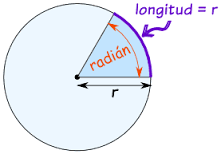
\includegraphics[width=\linewidth]{radian.png}
  \end{center}
\end{wrapfigure}
Los radianes no llevan un símbolo para identificarlos, y son MUY utilizados en el área científica como la forma mas común de medir ángulos a la hora de hacer cuentas.

Se llama radian al angulo que abarca un arco de circunferencia cuya longitud es igual al radio de la misma.


Por lo tanto, un circulo completo es un giro de ($2\pi $) radianes. Medio circulo ($180$) son $\pi$ radianes, un angulo recto son $\pi /2$ radianes, y así.

Vamos a ver que muchas veces los radianes son la forma mas cómoda para medir los ángulos.

\section*{Razones trigonométricas. Triangulo Rectángulo}

Pequeño repaso:
la suma de los ángulos internos de un triangulo suman $180\degree$.\\


\begin{minipage}{0.45\linewidth}

\begin{tikzpicture}[thick]
\coordinate (O) at (0,0);
\coordinate (A) at (3,0);
\coordinate (B) at (0,4);
\draw (O)--(A)--(B)--cycle;

\tkzLabelSegment[below=2pt](O,A){\textit{C.adyacente ('$b$')}}
\tkzLabelSegment[left=2pt](O,B){\textit{C. Opuesto ('$a$')}}
\tkzLabelSegment[above right=2pt](A,B){\textit{hipotenusa ('$h$')}}

\tkzMarkRightAngle[fill=orange,size=0.6,opacity=.4](A,O,B)% square angle here
\tkzLabelAngle[pos = 0.35](A,O,B){$\hat{\gamma}$}

\tkzMarkAngle[fill= orange,size=0.8cm,%
opacity=.4](B,A,O)
\tkzLabelAngle[pos = 0.6](B,A,O){$\hat{\alpha}$}

\tkzMarkAngle[fill= orange,size=0.8cm,%
opacity=.4](O,B,A)
\tkzLabelAngle[pos = 0.5](O,B,A){$\hat{\beta}$}

\end{tikzpicture}

\end{minipage}
\begin{minipage}{0.5\linewidth}
Teorema de pitagoras:
\[
a^2+b^2=h^2
\]

Hay tres razones trigonométricas principales que se definen como: %cambiar
\[
\sin(\hat{\alpha})=\frac{Cateto- opuesto}{hipotenusa}= \frac{a}{h}\]
\[
\cos(\hat{\alpha})=\frac{Cateto- adyacente}{hipotenusa}=\frac{b}{h}
\]
\[
\tan(\hat{\alpha})=\frac{Cateto- opuesto}{cateto- adyacente}=\frac{a}{b}
\]
\end{minipage}


Notar que lo que definimos como cateto opuesto o adyacente, depende del angulo que estemos usando ($\alpha$ en este caso).

Para $\beta$ el lado opuesto seria $b$ y el adyacente $a$.\\

Uso de la calculadora:
calcular senos y cosenos...
calcular los argumentos..

\href{http://tube.geogebra.org/m/960}{Versión interactiva de seno y coseno, como componentes de un triangulo rectangulo}

\href{}{Versión interactiva de seno y coseno como funciones de X}%variar parametros de sen y cos .

Las funciones como el seno o el coseno son muy importantes en una cantidad enorme de aplicaciones y modelos.

Las funciones trigonométricas fueron usadas ya por los antiguos griegos para deducir que la tierra era redonda, y calcular aproximadamente su radio. 
Hasta en la actualidad para calcular la posición de las cosas con los GPS, la posición de los satélites, o incluso la posición de los jugadores de fútbol cuando muestran una repetición por la tele.

También son muy importantes en muchos modelos de naturaleza, por ejemplo el sonido o la luz, que se comportan como ondas, se modelan con senos y cosenos.

Incluso son necesarios para entender como tecnologías como los cassetes y los vinilos hasta o los Blurays graban su información, y como funcionan las emisiones de radio o los rayos x.

Describir como oscila un péndulo o como rebota un resorte también da como resultado un seno o un coseno.

\section*{Teoremas del seno y coseno}

\begin{minipage}{0.45\linewidth}

\begin{tikzpicture}[thick]
\coordinate (O) at (0,0);
\coordinate (A) at (3.5,0);
\coordinate (B) at (-1,2.5);
\draw (O)--(A)--(B)--cycle;

\tkzLabelSegment[below=2pt](O,A){\textit{$b$}}
\tkzLabelSegment[left=2pt](O,B){\textit{$a$}}
\tkzLabelSegment[above right=2pt](A,B){\textit{$c$}}

\tkzMarkAngle[fill=orange,size=0.6,opacity=.4](A,O,B)% square angle here
\tkzLabelAngle[pos = 0.35](A,O,B){$\hat{a}$}

\tkzMarkAngle[fill= orange,size=0.8cm,%
opacity=.4](B,A,O)
\tkzLabelAngle[pos = 0.6](B,A,O){$\hat{b}$}

\tkzMarkAngle[fill= orange,size=0.7cm,%
opacity=.4](O,B,A)
\tkzLabelAngle[pos = 0.5](O,B,A){$\hat{c}$}

\end{tikzpicture}

\end{minipage}
\begin{minipage}{0.5\linewidth}
\textbf{Teorema del seno}:

\[
\frac{\bar{ab}}{\sin(\hat{c})}=\frac{\bar{ac}}{\sin(\hat{b})}=\frac{\bar{bc}}{\sin(\hat{a})}
\]

\textbf{Teorema del coseno}:

\[
\bar{ab}^2=\bar{ac}^2 + \bar{bc}^2 - 2.\bar{bc}.\bar{ac}.\cos(\hat{c})
\]

Se puede ver que el teorema de pitagóricas es un caso particular del teorema del coseno: si  $c=90 \degree$, entonces: 

..

..
\end{minipage}


\section*{Ejercicios}

Si se traban con algún ejercicio, pasen al siguiente, y vuelvan al ejercicio difícil mas tarde.szszszs



%cosas que voy a buscar: Raices, ordenadas al origen, asintotas. Dom, Im.
%Hacer algun multiple choice.

\section{Grados y Radianes}

Pasar de grados a radianes o viceversa, según corresponda.

\begin{enumerate}
\item 1 radian
\item $\frac{\pi}{3}$
\item $8\pi$
\item $3,5 rad$
\item $150\degree$
\item $60\degree$
\item $210\degree$
\item $315\degree$
\end{enumerate}

\section{completar:}

%\begin{table*}[ht!]
\begin{center}
%\caption{Completar}
\label{completar}
\begin{tabular}{|l|c|c|c|c|c|}
\hline
Radianes & 0 & $\frac{\pi}{6} $ & $\frac{\pi}{4} $ & $\frac{\pi}{3} $ & $\frac{\pi}{2} $ \Ts \Bs \\ \hline
Grados  &    &  &   &   &    \Ts \Bs     \\ \hline
\end{tabular}
%\end{table*}
\end{center}

\begin{center}
%\caption{Completar}
\label{completar}
\begin{tabular}{|l|c|c|c|c|c|c|c|}
\hline
Radianes &  &  &   &   &  &  & \Ts \Bs \\ \hline
Grados  & $300\degree$   & $150\degree$  & $90\degree$   & $30\degree$  & $45\degree$ &  $1\degree$ & $1250\degree$ \Ts \Bs     \\ \hline
\end{tabular}
%\end{table*}
\end{center}

\section{Demostrar}
$tg(\alpha)=a \Rightarrow \vert cos(\alpha).sen(\alpha)\vert =\frac{\vert a \vert}{a^2+1}$

\section{Resolver los siguientes triángulos rectángulos:}

\begin{tikzpicture}[thick]
\coordinate (O) at (0,0);
\coordinate (A) at (4,0);
\coordinate (B) at (0,2);
\draw (O)--(A)--(B)--cycle;

\tkzLabelSegment[below=2pt](O,A){\textit{adjacent leg}}
\tkzLabelSegment[left=2pt](O,B){\textit{opposite leg}}
\tkzLabelSegment[above right=2pt](A,B){\textit{hypotenuse}}

\tkzMarkRightAngle[fill=orange,size=0.5,opacity=.4](A,O,B)% square angle here
\tkzLabelAngle[pos = 0.35](A,O,B){$\gamma$}

\tkzMarkAngle[fill= orange,size=0.8cm,%
opacity=.4](B,A,O)
\tkzLabelAngle[pos = 0.6](B,A,O){$\alpha$}

\tkzMarkAngle[fill= grey,size=0.7cm,%
opacity=.4](O,B,A)
\tkzLabelAngle[pos = 0.5](O,B,A){$\beta$}

\end{tikzpicture}

\begin{enumerate}
\begin{multicols}{2}

\item $a=10cm$ $b=7cm$
\item $h=11cm$ $a=9cm$
\item $h=12cm$ $\sin (\alpha)=0,896$
\item $ $%quedan 4 mas almenos

\columnbreak

%problema de la isla

\end{multicols}
\end{enumerate} 

%f(x)=\frac{•}{•}

\section{Problemas}

\begin{enumerate}

\item Cual es el angulo de elevación del sol cuando un mástil de $24m$ proyecta una sombra de $16m$?
\item Cual es la altura de una antena si una persona que se encuentra a $250m$ de su base, observa su punta bajo un angulo de $22\degree$?
\item cual es el área de un pentágono regular de $40cm$ de perímetro?
\item cual es el área de un triangulo isósceles, cuya base mide 18cm y el angulo opuesto a ella mide $34\degree 50'$?
\item El perímetro de un triangulo isósceles es de 26cm y su base mide 10cm. cual es el valor de sus ángulos interiores?

\end{enumerate} 


\section{Ejemplo de Aplicación}

\rule[2ex]{\textwidth}{2pt}

Observación: Para saber si hiciste bien un ejercicio, reemplaza por tu valor de x.

%gifsicle --unoptimize animated.gif | convert - frame-%d.png
%\animategraphics[loop,autoplay]{12}{frame-}{0}{99}
\section*{Extra}

%El numero $e\simeq$ ..  breve bio de euler-
\begin{itemize}
\item Demostración del teorema de pitagoras:

\item Demostración de la relación pitagorica...%%??

\item Toda la geometría que vieron hasta ahora (desde la primaria) cae dentro de una rama de la geometría llamada geometría Eulidea o plana (en honor a Euclides).
Sin embargo existen otros tipos de geometrías, en las cuales pasan cosas a las que no estamos acostumbrados.
Por ejemplo que dos rectas paralelas se toquen, o que la suma  de los ángulos internos de un triangulo sumen mas o menos de 180 grados.
Estas geometrías se llaman geometrías de Riemman o curvas (En honor a Riemman, discípulo de Gauss).

Por ejemplo, dibujar un triangulo que empiece en el polo de la tierra y siga dos latitudes, arma un triangulo cuyos lados internos suman 270 grados.


\end{itemize}

%\bibliographystyle{plain}
%\bibliography{references}

%
%\newpage
%
%\section*{Resultados}
%\begin{enumerate}
%\item
%\begin{enumerate}
%\item -7 ; \item 16 ; \item .. ; \item $3/5$ ; \item 25 ; \item $64/9$ ; \item $c^b $ ;\item $k$ ;\item $\frac{b.d}{c^h} $  ;\item $b=1/c$ ;\item  $2.2,3$ ;\item $2-2,3 = 0,3$ ;\item 2,3/2 ;\item  4,6 ;\item 1$/2,3$ ;\item m/n ;\item  ; 
%\end{enumerate}
%
%\item 
%\begin{enumerate}
%\item
%\item
%\item $log_3(x+1)$
%\end{enumerate}
%
%\item
%\begin{enumerate}
%\item $x=8$
%\item $-2/3$
%\item $x=5$
%\item $x=9$
%\item 
%\item 
%\item $x=2$
%\item $x=2$
%\item $x=1$,$x=$ 
%\end{enumerate}
%
%\item
%
%\item 
%
%
%\end{enumerate}

\end{document}